\subsection*{Convolutional VAE}
The convolutional VAE is implemented in the file \texttt{density\_modeling.ipynb} by extending the encoder and decoder of the original VAE with convolutional layers. The encoder portion of the network uses a series of convolutional layers (Conv2d) with kernel size 4, stride 2, and padding 1. These layers take in a single-channel image and output 32, 64, and 128 channels, respectively. Since the stride is 2, the output of each layer is half the size of the input. The output of these layers is then flattened and passed through a linear layer with 100 units to produce the encoded representation of the input image. This encoded representation is then passed through two linear layers to produce the mean and variance of the latent space, respectively.

The decoder portion of the network takes in the latent space and passes it through a linear layer with 100 units to produce the decoder's input. This input is then passed through a linear layer with 12833 units, which reshapes the input to match the shape of the output from the encoder. The output is then passed through a series of transposed convolutional layers (ConvTranspose2d) with kernel size 4, stride 2, and padding 1, which take in 128, 64, and 32 channels, respectively, and output a single-channel image. The output of the final layer is passed through a sigmoid activation function to produce the final output image. We expect that the quality of the model will be better than the original VAE since convolutional layers are usually more suited for image data and can capture spatial hierarchies and patterns in the data that linear layers are not able to.

The parameters of the network were estimated using the Adam optimizer and the ELBO loss. ELBO is the sum of two terms: the reconstruction loss (BCE) and the KL divergence. By minimizing this loss, the VAE can learn a good approximation of the true posterior and generate realistic samples from the learned latent space. Both models were trained for 100 epochs with a batch size of 128. The models were trained with a learning rate of 0.0005 and a weight decay of 0. We trained both models on the MNIST dataset with a varying number of latent dimensions. The results are shown in Figure~\ref{fig:vaeloss}.

\begin{figure}[h]
\centering
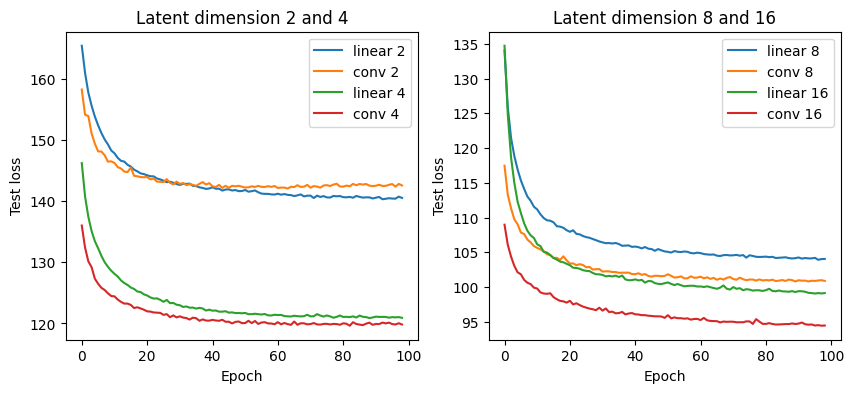
\includegraphics[width=\textwidth]{images/test_loss.png}
\setlength{\belowcaptionskip}{-10pt}
\caption{ELBO reconstruction loss on test set for VAE and Convolutional VAE with varying number of latent dimensions.}
\label{fig:vaeloss}
\end{figure}

\begin{table}
\centering
\begin{tabular}{|c|c|c|}
\hline
\multicolumn{1}{|c|}{\textbf{Latent Dimensions}} & \multicolumn{1}{c|}{\textbf{Original VAE}} & \multicolumn{1}{c|}{\textbf{Convolutional VAE}} \\ \hline
\multicolumn{1}{|c|}{2} & \multicolumn{1}{c|}{140.54} & \multicolumn{1}{c|}{142.58}  \\ \hline
\multicolumn{1}{|c|}{4} & \multicolumn{1}{c|}{120.92} & \multicolumn{1}{c|}{119.83}  \\ \hline
\multicolumn{1}{|c|}{8} & \multicolumn{1}{c|}{104.03} & \multicolumn{1}{c|}{100.86}  \\ \hline
\multicolumn{1}{|c|}{16} & \multicolumn{1}{c|}{99.117} & \multicolumn{1}{c|}{94.446}  \\ \hline
\multicolumn{1}{|c|}{32} & \multicolumn{1}{c|}{99.136} & \multicolumn{1}{c|}{94.434}  \\ \hline
\end{tabular}
\vspace*{0.5cm}
\setlength{\belowcaptionskip}{-10pt}
\caption{ELBO reconstruction loss on test set for VAE and Convolutional VAE with varying number of latent dimensions.}
\label{tab:vaeloss}
\end{table}

We see that the original VAE performs better than the convolutional VAE for the 2-dimensional latent space. The difference is not significant, but it is still interesting to note. One explanation for this would be that the original VAE can learn a simpler, more linear structure of the data when the latent dimensions are low. This structure is sufficient to capture the information in the MNIST dataset. However, as the latent dimensions rise, the initial VAE finds it harder to understand a more intricate, non-linear data structure.

Contrarily, convolutional VAEs can learn spatial hierarchies in the data and is meant to handle high-dimensional data, such as images. As a result, it can still function more effectively when the latent dimensions are larger. Hence, the convolutional VAE performs better than the original VAE for all other latent dimensions (4, 8, 16, 32).

The difference between 16 and 32 latent dimensions for each of the models among themselves is minimal, hence why we do not show results for 32 latent dimensions in the graph. Surprisingly, we did not see a significant improvement from 16 to 32 latent dimensions in the convolutional VAE. We think this is because the convolutional VAE is not large enough to capture the information in the data. The convolutional VAE is a relatively small network, and it is possible that it is not able to learn the complex structure of the data with 32 latent dimensions.

We are confident that a convolutional VAE could perform better than the original VAE when the latent dimensions are two if we adjust the network's capacity and use techniques such as batch normalization and dropout. If we increase the network size, we also expect that the convolutional VAE will have a more significant difference in performance between 16 and 32 latent dimensions.

We can also compare the performance of the original VAE and convolutional VAE by looking at the reconstructions visualized in Figure~\ref{fig:reconstructions}. We use the models trained with 16 latent dimensions to generate the reconstructions. We see that the original VAE can reconstruct the images reasonably well, but the convolutional VAE can reconstruct the images more accurately.


\begin{figure}[h]
    \centering
    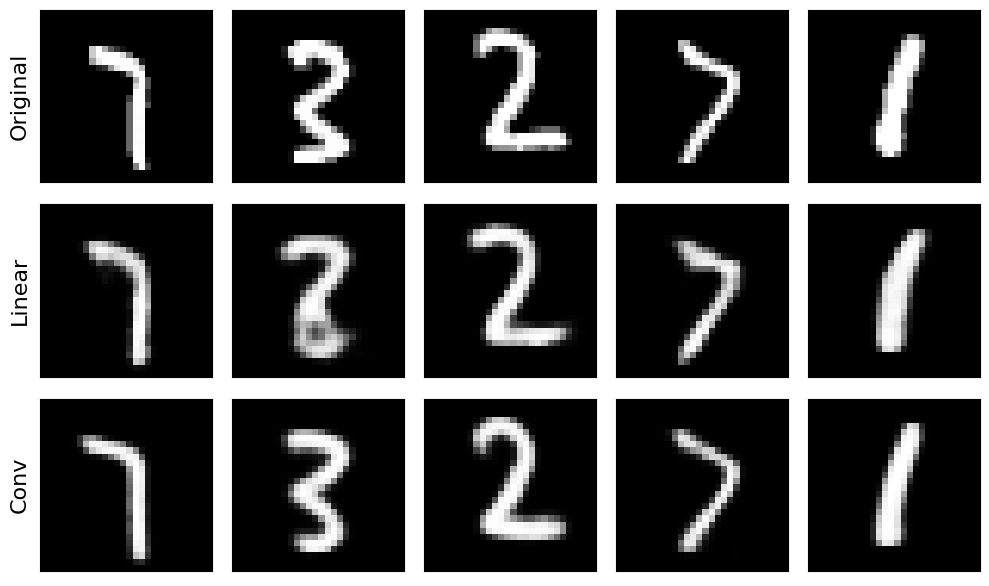
\includegraphics[width=11cm]{images/reconstructions.png}
    \setlength{\belowcaptionskip}{-10pt}
    \caption{Reconstructions of the original VAE and convolutional VAE. Latent dimensions = 16.}
    \label{fig:reconstructions}
\end{figure}

\subsection*{Diffusion model}

We have implemented a Diffusion model to generate images from the MNIST dataset. The model is based on the paper \cite{diffusion} and is a generative model that uses a diffusion process to generate images. Diffusion models are a class of generative models that have recently established themselves as state-of-the-art in image generation with popular models such as DALL-E-2, stable diffusion, and midjourney.

Diffusion models define a markov chain of diffusion steps, where at each step we add random noise to the image and the learn the reverse process. Therefore, they are able to model complex distributions of images and have proven to be very effective in generating realistic images.

However, one disadvantage of diffusion models is that they can be more difficult to implement, train, and optimize as opposed to other models such as VAEs. This is because they are based on a continuous-time stochastic process, and the optimization of the model is not as straightforward as it is for VAEs. Training a diffusion model can also be computationally expensive, and it can take a long time to train it to generate high-quality images.

In the forward process we gradually add gaussian noise to the image according to a variance schedule $\beta_1, \vdots, \beta_T$. The diffusion process is defined as follows:
\begin{align*}
    q\left(\mathbf{x}_t \mid \mathbf{x}_{t-1}\right):=\mathcal{N}\left(\mathbf{x}_t ; \sqrt{1-\beta_t} \mathbf{x}_{t-1}, \beta_t \mathbf{I}\right)
\end{align*}

where $\mathbf{x}_t$ is the image at time $t$ and $\mathbf{x}_{t-1}$ is the image at time $t-1$. The paper \cite{diffusion} states that the forward process variances $\beta_t$ can be learned or fixed. We have fixed the variances to be linarly spaced between $10^{-4}$ and $0.02$, and we have used 1000 diffusion steps $T$. These are the same values that were used in the paper \cite{diffusion}. The reverse process of the difussion is defined as follows:

\begin{align*}
    p_\theta\left(\mathbf{x}_{t-1} \mid \mathbf{x}_t\right)&=\mathcal{N}\left(\mathbf{x}_{t-1} ; \boldsymbol{\mu}_\theta\left(\mathbf{x}_t, t\right), \boldsymbol{\Sigma}_\theta\left(\mathbf{x}_t, t\right)\right)\\
    p_\theta\left(\mathbf{x}_{0: T}\right)&=p\left(\mathbf{x}_T\right) \prod_{t=1}^T p_\theta\left(\mathbf{x}_{t-1} \mid \mathbf{x}_t\right)\\
    p_\theta\left(\mathbf{x}_0\right) &=\int p_\theta\left(\mathbf{x}_{0: T}\right) d \mathbf{x}_{1: T}
\end{align*}

Here we have that $\theta$ is the parameters we train. We use a simple Unet to trainrepresent the reverse process and we use the ELBO loss function to train the model. The represent time, we use the  Transformer sinusoidal position embedding as described in the paper \cite{diffusion}. However, we apply no self-attention. Our Unet is very simple and will very likely not be able to compete with the more complex Unets used in the paper \cite{diffusion}. We tried using a simpler arcitecture, but the results were not nearly as good. We use the Adam optimizer with a learning rate of $10^{-4}$ and a batch size of 128. We train the model for 100 epochs.

\begin{figure}[h]
    \centering
    \subfloat[\centering Diffusion]{{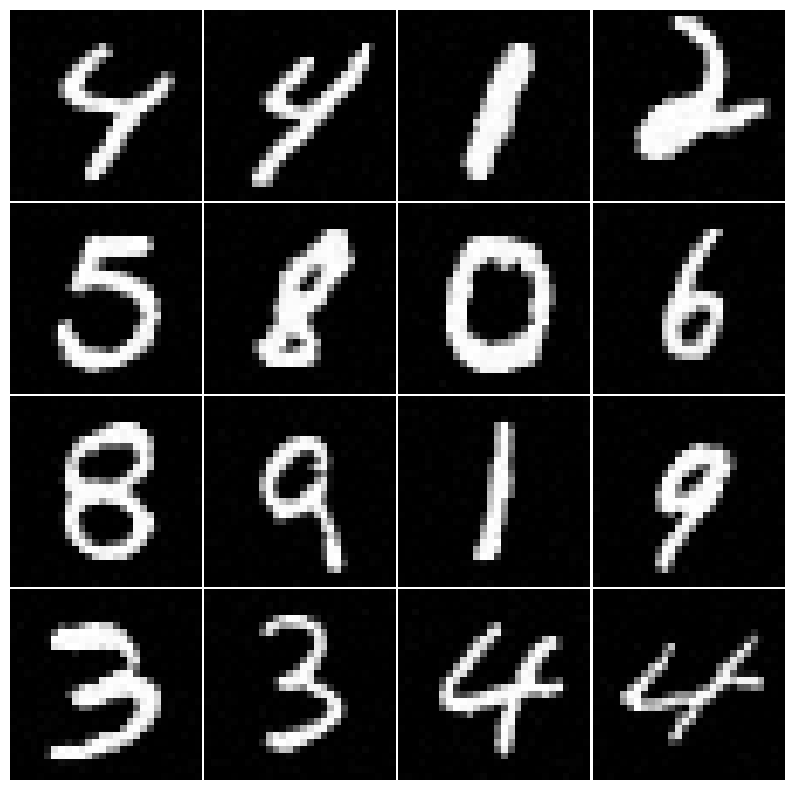
\includegraphics[width=6.5cm]{images/diffusion.png} }}%
    \subfloat[\centering Original VAE]{{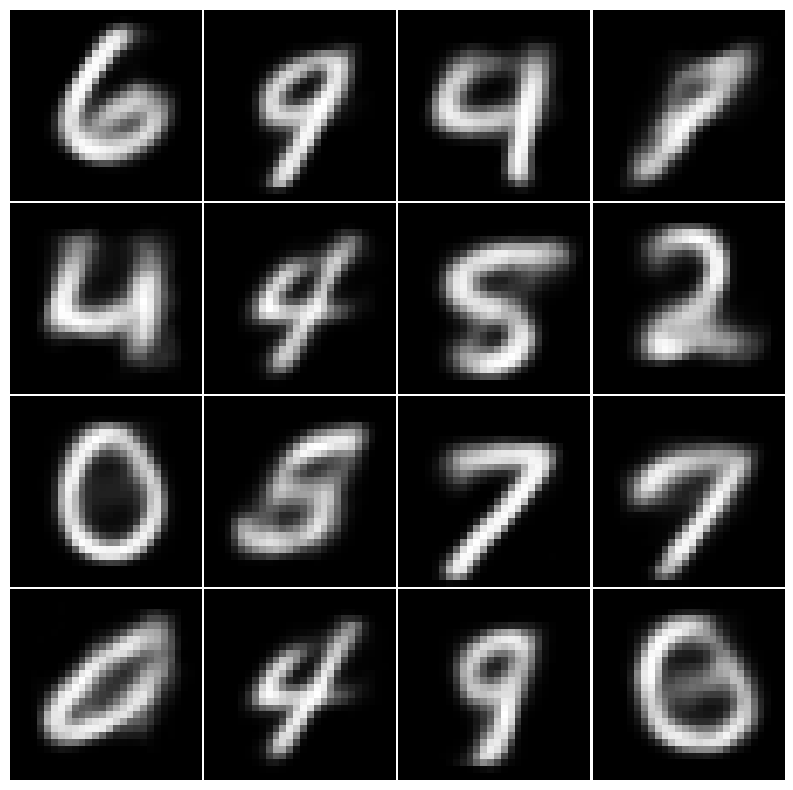
\includegraphics[width=6.5cm]{images/vae_sample.png} }}%
    \setlength{\belowcaptionskip}{-10pt}
    \caption{Comparison of generated images from the diffusion model and the original VAE.}
    \label{fig:example}%
\end{figure}

To compare this model with the original VAE generate 100 images from the original VAE and 100 images from the diffusion model. With the VAE we generate images by generating two latent variables and then using the decoder to generate an image. With the diffusion model we generate images starting with an image with random noise and use the reverse process to generate an image. We then compare the images generated by the two models with Fréchet inception distance (FID). FID is a metric used to evaluate the quality of generated images in generative models, such as Diffusion models and GANs. It measures the distance between feature representations of real and generated images in a feature space defined by an inception network (a pre-trained convolutional neural network). The lower the FID score, the more similar the real and generated images are, and the better the generative model is at producing realistic images. We use the test set of the MNIST dataset to calculate the FID score. The diffusion network achives a FID score of 0.0115, while the original VAE achives a FID score of 0.2689. This means that the distribution of the images generated by the diffusion model is much closer to the distribution of the real images. We can also visualize the images generated by the two models in Figure~\ref{fig:example}. We see that the images generated by the diffusion model are much more realistic than the images generated by the original VAE.
